\chapter{Ongeslachtelijke voortplanting en klonen bij planten}\label{ch:b2:asexual-reproduction}

In een dal in Utah staat een bos van zevenenveertigduizend
populierenstammen dat één plant is: elke stam is gegroeid uit hetzelfde
wortelstelsel, elke cel draagt hetzelfde genoom, en het individu is zo'n
veertienduizend jaar oud en weegt zesduizend ton. Elke aardbei in een
supermarktbakje van één ras is een stukje van één plant, vermeerderd via
uitlopers; elke cavendishbanaan op aarde is een stek van een stek van één
plant. Planten kunnen, anders dan de meeste dieren, zonder seks nieuwe
individuen maken --- uit een stengel, een wortel, een blad, één enkele cel
in een kolf. Dit hoofdstuk onderzoekt hoe ze dat doen, hoe telers er
gebruik van maken, en wat het een lijn kost om \omterm{def:b2:meiosis-heredity:meiosis}{meiose} en bevruchting op te
geven: de vraag waarom seks überhaupt bestaat.

\section{Vegetatieve vermeerdering}

\begin{definition}[Kloon, genet, ramet]\label{def:b2:asexual-reproduction:clone}
\index{kloon}\index{genet}\index{ramet}\index{vegetatieve vermeerdering}
\emph{Ongeslachtelijke voortplanting} brengt uit één ouder nieuwe
individuen voort door mitose alleen, zonder \omterm{def:b2:meiosis-heredity:meiosis}{meiose} of bevruchting: de
nakomelingen vormen een \emph{kloon}, genetisch identiek aan de ouder en
aan elkaar, afgezien van de somatische \omterm{def:b2:genome-diversification:mutation}{mutaties} die zich opstapelen. Bij
planten is de gewone vorm de \emph{vegetatieve vermeerdering}, waarbij een
deel van het lichaam --- stengel, wortel, blad --- wortel schiet en een
aparte plant wordt. Een \emph{genet} is het genetische individu, alles wat
uit één zygote is gegroeid; een \emph{ramet} is een fysiologisch
afzonderlijke eenheid daarvan. Een aardbeienbed kan duizend rameten van één
genet bevatten; het populierenbos is één genet. Vegetatieve vermeerdering
is mogelijk omdat plantencellen het vermogen behouden om zich te delen en
elk orgaan te vormen --- ze zijn \emph{totipotent} --- en omdat planten
groeien vanuit meristemen die bijna overal opnieuw kunnen worden gewekt.
\end{definition}

\begin{proposition}[De organen van vegetatieve vermeerdering]\label{prop:b2:asexual-reproduction:organs}
\index{uitloper}\index{wortelstok}\index{knol}\index{bol}
Planten hebben dezelfde truc vanuit elk orgaan ontwikkeld. Vanuit
stengels: \emph{uitlopers} of \emph{stolonen}, horizontale scheuten langs
de grond die op hun knopen wortel schieten (aardbei, kruipende
boterbloem); \emph{wortelstokken}, horizontale ondergrondse stengels die
vertakken en in stukken uiteenvallen (kweekgras, iris, gember,
adelaarsvaren); \emph{knollen}, verdikte uiteinden van wortelstokken die
zetmeel opslaan en knoppen dragen, de ``ogen'' (aardappel);
\emph{bolknollen}, verdikte rechtopstaande stengelbases (krokus);
\emph{broedbolletjes}, kleine bolletjes die in de bladoksels of in de
bloeiwijze ontstaan (knoflook, sommige uien). Vanuit bladeren:
\emph{bollen}, knoppen omwikkeld door vlezige opslagbladeren die zich in
dochterbollen splitsen (ui, tulp); plantjes langs de bladrand, compleet met
wortels, die afvallen (\emph{Kalanchoe}). Vanuit wortels:
\emph{wortelopslag}, scheuten die uit horizontale wortels opschieten
(ratelpopulier, sleedoorn, framboos). Door \emph{fragmentatie}: een stuk
wilgentak dat wegdrijft en wortel schiet, een blaadje eendenkroos dat zich
splitst. In elk geval wordt een opslagorgaan of een meristeem over een
korte afstand meegevoerd, en begint de dochter haar leven met een
voedselvoorraad die geen \omterm{def:b2:angiosperm-reproduction:seed}{zaad} kan evenaren.
\end{proposition}

\begin{omfigure}
\begin{tikzpicture}[every node/.style={font=\scriptsize}]
  % runner
  \begin{scope}
    \draw[thick] (0,0) -- (3.6,0);
    \foreach \x in {0,1.8} { \draw[thick, omExo!70!black, fill=omExo!30] (\x,0) .. controls (\x-0.3,0.6) and (\x+0.3,0.6) .. (\x,0); \foreach \a in {60,90,120} \draw[thick, omExo!70!black] (\x,0) -- ++(\a:0.7); \draw[gray] (\x,0) -- ++(-100:0.4) (\x,0) -- ++(-70:0.4); }
    \draw[thick, omThm] (0.2,0.15) .. controls (0.9,0.55) and (1.2,0.55) .. (1.8,0.1);
    \draw[thick, omThm] (2.0,0.15) .. controls (2.7,0.55) and (3.0,0.55) .. (3.5,0.1);
    \draw[thick, omExo!70!black] (3.5,0.1) -- ++(80:0.4); \draw[gray] (3.5,0.1) -- ++(-80:0.3);
    \node[below, align=center] at (1.8,-0.55) {uitloper (aardbei):\\een horizontale scheut schiet wortel op zijn knopen};
  \end{scope}
  % rhizome and tuber
  \begin{scope}[xshift=5.2cm]
    \draw[gray, dashed] (-0.2,0) -- (3.8,0);
    \draw[very thick, omProp!80!black] (0,-0.5) -- (3.4,-0.5);
    \foreach \x in {0.6,2.0} \draw[thick, omExo!70!black] (\x,-0.5) -- (\x,0.7) (\x,0.3) -- ++(40:0.4) (\x,0.3) -- ++(140:0.4);
    \draw[thick, omProp!80!black, fill=omProp!40] (3.4,-0.5) ellipse (0.45 and 0.3);
    \foreach \p in {(3.2,-0.3),(3.6,-0.35),(3.7,-0.6)} \fill[omThm] \p circle (0.04);
    \foreach \x in {0.3,1.3,2.5} \draw[gray] (\x,-0.5) -- (\x,-0.9);
    \node[below, align=center] at (1.8,-1.05) {wortelstok en knol (aardappel):\\ondergrondse stengels,\\knoppen (ogen) op de knol};
  \end{scope}
  % bulb
  \begin{scope}[xshift=12.2cm]
    \draw[thick, fill=omExo!15] (0,-0.9) .. controls (-0.9,-0.6) and (-0.9,0.9) .. (0,1.0) .. controls (0.9,0.9) and (0.9,-0.6) .. (0,-0.9);
    \foreach \r in {0.55,0.35} \draw[thick] (0,-0.75) .. controls (-\r,-0.5) and (-\r,0.6) .. (0,0.8) .. controls (\r,0.6) and (\r,-0.5) .. (0,-0.75);
    \fill[omExo!60!black] (-0.1,-0.75) rectangle (0.1,0.3);
    \draw[thick, omThm, fill=omThm!30] (0.35,-0.5) ellipse (0.15 and 0.3);
    \foreach \x in {-0.3,0,0.3} \draw[gray] (\x,-0.9) -- (\x,-1.25);
    \node[below, align=center] at (0,-1.3) {bol (ui):\\vlezige bladeren,\\een dochterbol (rood)};
  \end{scope}
\end{tikzpicture}

{\small Drie organen van \omterm{def:b2:asexual-reproduction:clone}{vegetatieve vermeerdering}: uitlopers die op hun
knopen wortel schieten, een ondergrondse stengel die tot een knol
opzwelt, en een bol die een dochterbol vormt. In elk geval reist een knop
met zijn voedsel mee.}
\end{omfigure}

\begin{omfigure}
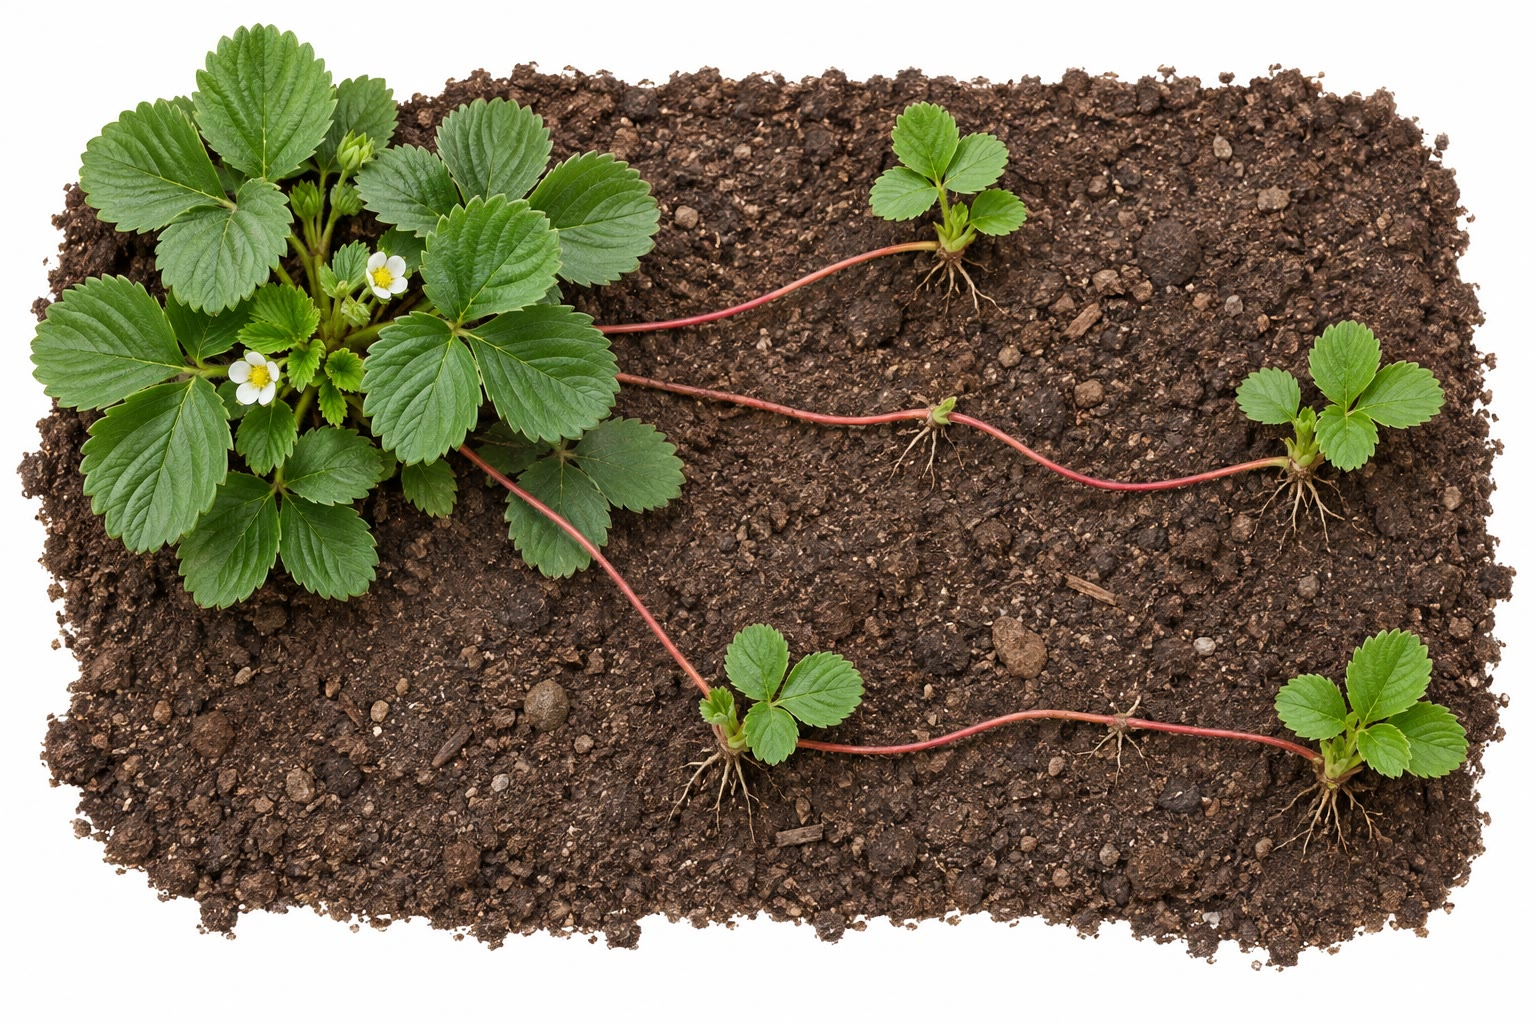
\includegraphics[width=0.46\linewidth]{images/book4/ai/b4-07-strawberry-runners.jpg}\hspace{0.03\linewidth}
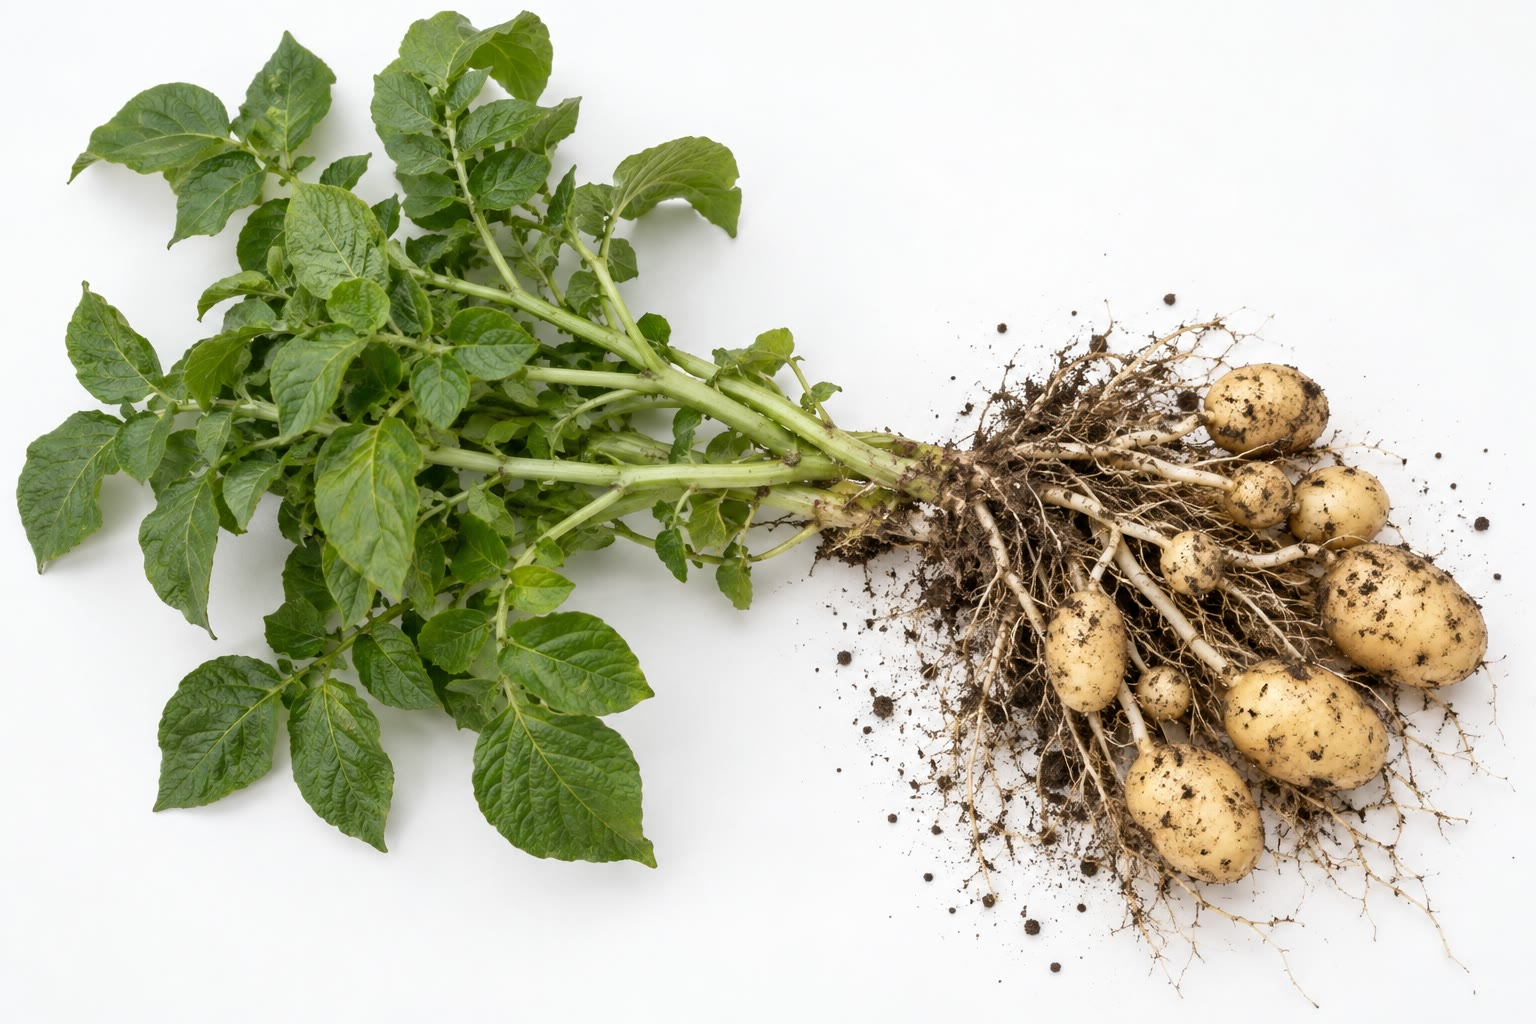
\includegraphics[width=0.46\linewidth]{images/book4/ai/b4-07-potato-tubers.jpg}

{\small Links: een aardbeienplant en de dochterplanten die langs haar
uitlopers wortel schieten. Rechts: een uit de grond gehaalde
aardappelplant, met haar knollen aan stolonen --- elke knol een stuk
stengel dat zal uitgroeien tot een plant die genetisch identiek is aan
deze.}
\end{omfigure}

\begin{theorem}[De meetkunde van een zich uitbreidende kloon]\label{thm:b2:asexual-reproduction:spread}
\index{klonale groei}
Een \omterm{def:b2:asexual-reproduction:clone}{genet} waarvan elke \omterm{def:b2:asexual-reproduction:clone}{ramet} per jaar $m$ bewortelde dochters voortbrengt,
die allemaal overleven, groeit in aantal als $N(t) = N_0 (1 + m)^t$ ---
exponentiële groei zonder enige seks --- totdat de \omterm{def:b2:asexual-reproduction:clone}{rameten} de ruimte vullen
bij hun draagdichtheid $d$ (\omterm{def:b2:asexual-reproduction:clone}{rameten} per oppervlakte-eenheid), waarna de
\omterm{def:b2:asexual-reproduction:clone}{kloon} als een front oprukt. Een \omterm{def:b2:asexual-reproduction:clone}{kloon} die zijn uitlopers in een rechte
lijn met snelheid $v$ uitzendt, heeft na $t$ jaar een straal $vt$, en het
aantal \omterm{def:b2:asexual-reproduction:clone}{rameten} groeit als $\pi d (vt)^2$: kwadratisch, niet exponentieel.
Een aardbeienplant die haar uitlopers \qty{0.5}{m} per jaar uitzendt,
heeft na tien jaar een straal van \qty{5}{m}; de populierenkloon uit de
openingsalinea, \qty{43}{ha}, heeft een straal van zo'n \qty{370}{m}
en, bij een netto opmars van enkele centimeters per jaar, een
leeftijd in de orde van $10^{4}$ jaar --- in overeenstemming met de
leeftijd die uit de terugtrekking van de gletsjers is geschat.
\end{theorem}
\begin{proof}
Elk jaar wordt elke \omterm{def:b2:asexual-reproduction:clone}{ramet} vervangen door zichzelf plus $m$ dochters, een
factor $1 + m$; $t$ jaar geven $(1 + m)^t$. Zodra het binnenste vol is,
vinden alleen de \omterm{def:b2:asexual-reproduction:clone}{rameten} aan de rand nog ruimte, en de rand rukt op met
de snelheid $v$ van de uitlopers; de oppervlakte is $\pi(vt)^2$ en het
aantal \omterm{def:b2:asexual-reproduction:clone}{rameten} is de oppervlakte maal de dichtheid.
\end{proof}

\begin{example}[De oudste organismen]\label{ex:b2:asexual-reproduction:oldest}
De populierenkloon Pando (Utah) beslaat \qty{43}{ha} met ongeveer
\num{47000} stammen die elk een eeuw of zo leven en worden vervangen door
wortelopslag uit dezelfde wortels; het \omterm{def:b2:asexual-reproduction:clone}{genet} kan meer dan tienduizend jaar
oud zijn. Een \omterm{def:b2:asexual-reproduction:clone}{kloon} van het zeegras \emph{Posidonia} in de Middellandse
Zee strekt zich over \qty{15}{km} uit en kan honderdduizend jaar oud zijn;
een ring van creosootstruiken in de Mojavewoestijn is gedateerd op
\num{11700} jaar, waarbij de centrale stengels afsterven terwijl de ring
zich uitbreidt. Wat oud is, is telkens het \omterm{def:b2:asexual-reproduction:clone}{genet}; geen enkele cel erin is
ouder dan enkele decennia, en het genoom is duizenden keren gekopieerd.
\end{example}

\section{Zaden zonder seks, en dieren zonder vaders}

\begin{definition}[Apomixie]\label{def:b2:asexual-reproduction:apomixis}
\index{apomixie}\index{parthenogenese}
\emph{Apomixie} is de vorming van zaden zonder bevruchting: een embryo
ontwikkelt zich uit een ongereduceerde eicel (de megasporemoedercel slaat
de \omterm{def:b2:meiosis-heredity:meiosis}{meiose} over) of rechtstreeks uit een cel van de nucellus, en het \omterm{def:b2:angiosperm-reproduction:seed}{zaad}
draagt het \omterm{def:b2:meiosis-heredity:vocabulary}{genotype} van de moeder. Paardenbloemen, havikskruiden,
bramen, veldbeemdgras en veel citrussoorten doen dit; het citruszaad
bevat vaak meerdere embryo's, één geslachtelijk en de rest nucellaire
kopieën van de moeder. Apomixie behoudt het \omterm{def:b2:angiosperm-reproduction:seed}{zaad} --- zijn verspreiding,
\omterm{def:b2:angiosperm-reproduction:seed}{kiemrust} en \omterm{def:b2:angiosperm-reproduction:seed}{zaadhuid} --- en laat de \omterm{def:b2:meiosis-heredity:meiosis}{meiose} vallen, zodat een goed
aangepast \omterm{def:b2:meiosis-heredity:vocabulary}{genotype} ongewijzigd wordt verspreid; de meeste apomicten zijn
\omterm{def:b2:genome-diversification:polyploidy}{polyploïden} van hybride oorsprong, bij wie de \omterm{def:b2:meiosis-heredity:meiosis}{meiose} toch zou mislukken.
De dierlijke tegenhanger is de \emph{parthenogenese}, de ontwikkeling uit
een onbevruchte eicel: obligaat bij sommige hagedissen en bij bdelloïde
raderdiertjes, die al tientallen miljoenen jaren geen mannetjes meer
hebben; cyclisch bij bladluizen en watervlooien, die zich de hele zomer
parthenogenetisch vermenigvuldigen, waarbij een vrouwtje levende dochters
baart die al hun eigen embryo's dragen, en die in de herfst overschakelen
op een geslachtelijke generatie die overwinterende eieren legt.
\end{definition}

\begin{omfigure}
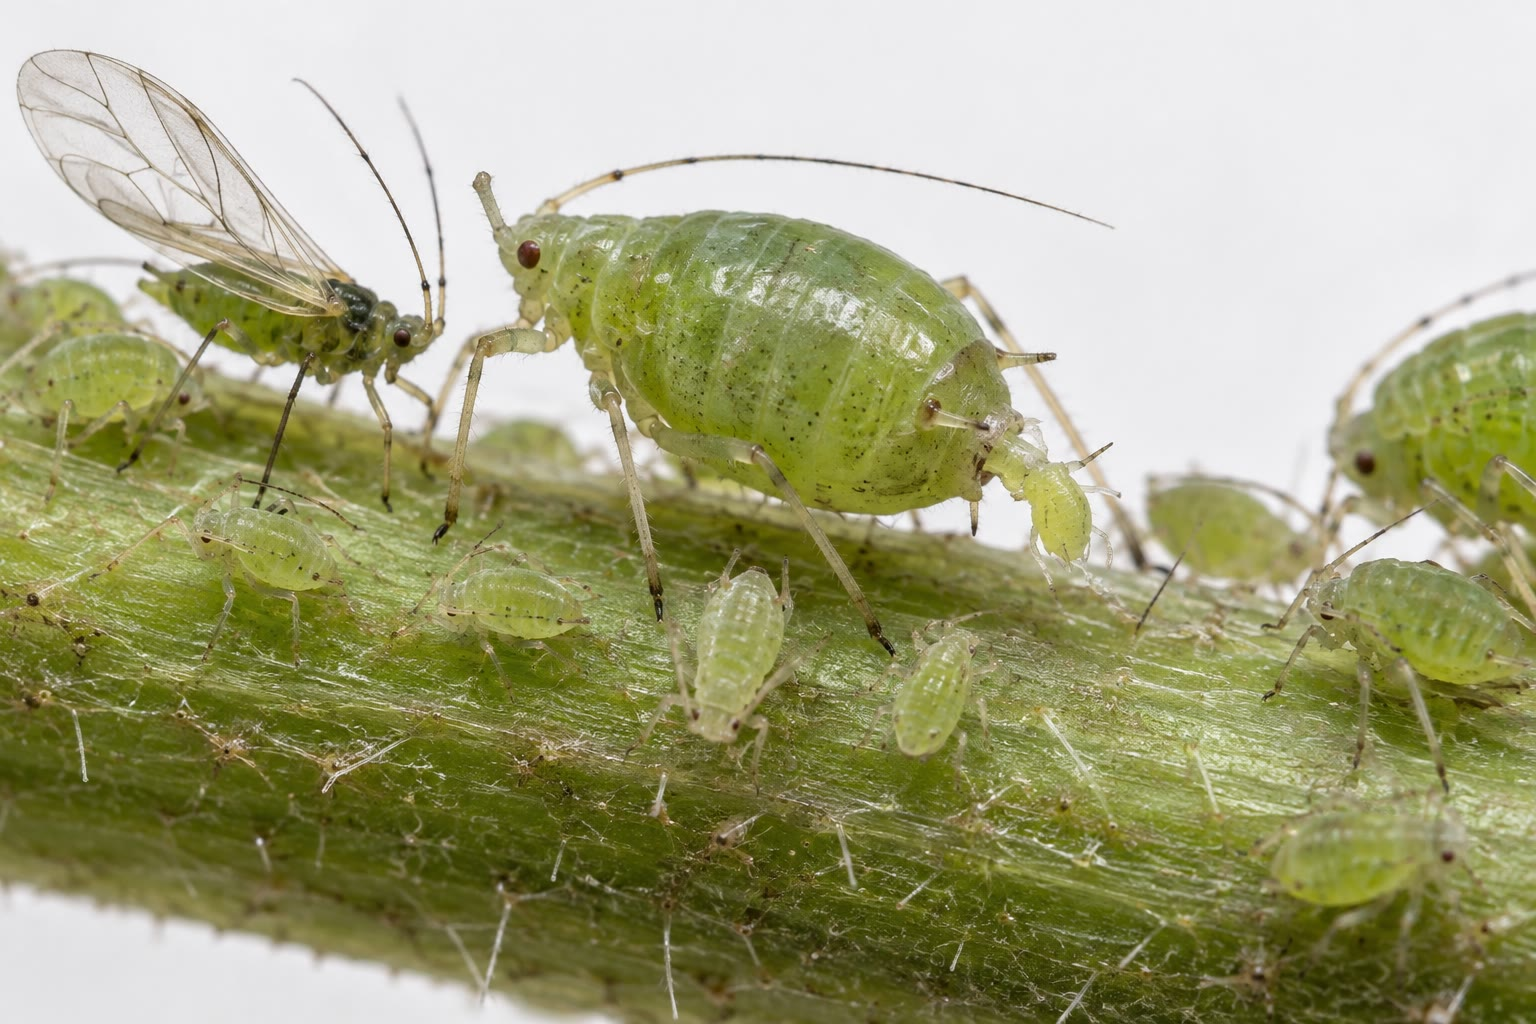
\includegraphics[width=0.55\linewidth]{images/book4/ai/b4-07-aphids.jpg}

{\small Bladluizen op een stengel: een ongevleugeld parthenogenetisch
vrouwtje dat een levende dochter baart, nimfen van verschillende
leeftijden, en een gevleugelde migrant --- een zomer vol exponentiële groei
zonder één enkel mannetje.}
\end{omfigure}

\begin{example}[Een zomer van bladluizen]\label{ex:b2:asexual-reproduction:aphids}
Een parthenogenetische bladluis wordt in ongeveer acht dagen volwassen en
brengt twee weken lang zo'n vijf dochters per dag voort; de dochters
worden al zwanger geboren (de embryo's beginnen zich te ontwikkelen in de
embryo's van de moeder). Met een \omterm{def:b2:unicellular-diversity:division}{generatietijd} van ongeveer tien dagen en
een netto vermenigvuldiging van ongeveer \num{50} per generatie zou één
stichtster in april, ongeremd, tegen oktober $50^{12} \approx 2\times 10^{20}$
nakomelingen kunnen nalaten --- een massa groter dan die van de aarde.
Lieveheersbeestjes, gaasvliegen, sluipwespen, schimmels en regen houden
het aantal op enkele duizenden per plant, en de geslachtelijke generatie
in de herfst zet de \omterm{def:b2:asexual-reproduction:clone}{kloon} vóór de winter terug in gerecombineerde eieren.
\end{example}

\section{Klonen door de teler}

\begin{proposition}[Stekken, afleggen, enten]\label{prop:b2:asexual-reproduction:horticulture}
\index{stek}\index{enten}\index{onderstam}
Een \emph{stek} is een stuk stengel, wortel of blad dat men wortel laat
schieten: het afgesneden uiteinde vormt een callus van delende cellen
waaruit wortelmeristemen ontstaan, geholpen door auxine (het
bewortelingshormoon) en vochtigheid. Bij \emph{afleggen} laat men een tak
wortel schieten terwijl hij nog vastzit, en snijdt men hem daarna los. Bij
\emph{enten} wordt een scheut van de ene plant (de \emph{ent}) verbonden
met de bewortelde stengel van een andere (de \emph{onderstam}): de twee
cambia worden tegen elkaar gedrukt, callus overbrugt de wond, en binnen
enkele weken verbinden nieuw xyleem en floëem beide delen. De geënte plant
is een chimaera --- de wortels behouden het genoom van de onderstam, de
vruchtdragende scheut dat van de ent --- en enten werkt alleen tussen
verwante planten (soorten van één geslacht, soms van één familie), omdat de
weefsels elkaars cellen moeten herkennen. Elk ras van appel, peer, kers,
citrus en druif wordt door enten vermeerderd: een benoemd ras is één
\omterm{def:b2:asexual-reproduction:clone}{genet}, dat eeuwenlang door enten in leven wordt gehouden (de
reinetteappels dateren uit de zestiende eeuw), en de onderstam wordt
gekozen op grond van de bodem, de ziekte en de gewenste boomgrootte ---
zwakgroeiende onderstammen geven de kleine bomen van moderne boomgaarden.
\end{proposition}

\begin{proposition}[Microvermeerdering en totipotentie]\label{prop:b2:asexual-reproduction:tissueculture}
\index{microvermeerdering}\index{totipotentie}\index{callus}
Elke levende plantencel met een kern kan in principe een hele plant
regenereren. In \emph{weefselkweek} wordt een gesteriliseerd stukje weefsel
(een \emph{explantaat}: een scheuttop, een bladschijfje, een helmknop) op
een agarmedium met suiker, mineralen, vitaminen en hormonen geplaatst. Met
auxine en cytokinine in evenwicht dedifferentiëren de cellen tot een
\emph{callus}, een massa delende ongespecialiseerde cellen; met meer
cytokinine dan auxine vormt het callus scheuten, met meer auxine dan
cytokinine vormt het wortels, en bij sommige soorten vormt het
\emph{somatische embryo's} --- volledige embryo's zonder eicel. Scheuten
worden om de paar weken afgesneden en overgezet, waarbij ze telkens met
een factor drie tot tien vermenigvuldigen, zodat één meristeem in een jaar
een miljoen plantjes geeft. Omdat virussen achterblijven bij de groeiende
top, is een scheutmeristeem van minder dan een millimeter lang zelfs in een
geïnfecteerde plant meestal virusvrij: \emph{meristeemcultuur} is de manier
waarop uitgangsmateriaal van aardappel, aardbei, banaan en orchidee wordt
gezuiverd. De methode is het praktische bewijs van totipotentie, en de
reden waarom een plantenras binnen enkele jaren na zijn ontstaan bij
miljoenen kan worden verkocht.
\end{proposition}
\begin{proof}[Bewijsmateriaal]
Skoog en Miller (1957) kweekten callus uit tabaksmerg op media met
verschillende verhoudingen van auxine tot het pas ontdekte cytokinine: veel
auxine gaf wortels, veel cytokinine gaf scheuten, een evenwicht gaf alleen
callus --- de orgaanvorming werd bepaald door de verhouding van twee
hormonen, niet door een specifieke orgaanvormende stof. Steward (1958)
bracht afzonderlijke cellen en kleine klompjes uit een wortel van een peen
in suspensie in een draaiende kolf met kokosmelk: sommige klompjes vormden
embryoachtige structuren die uitgroeiden tot volledige, bloeiende penen,
wat aantoonde dat een gedifferentieerde cel van een volwassen orgaan nog
het hele ontwikkelingsprogramma bezit en kan gebruiken.
\end{proof}

\begin{omfigure}
\begin{tikzpicture}[every node/.style={font=\scriptsize}, >=stealth]
  \node[draw, rounded corners, fill=omDef!12, align=center] (ex) at (0,0) {explantaat\\(scheuttop, bladschijfje)};
  \node[draw, rounded corners, fill=omExo!30, align=center] (cal) at (4.6,0) {callus\\auxine $\approx$ cytokinine};
  \node[draw, rounded corners, fill=omExo!30, align=center] (sh) at (8.4,1.2) {scheuten\\cytokinine $>$ auxine};
  \node[draw, rounded corners, fill=omExo!30, align=center] (rt) at (8.4,-1.2) {wortels\\auxine $>$ cytokinine};
  \node[draw, rounded corners, fill=omDef!12, align=center] (pl) at (12.2,0) {plantjes\\geacclimatiseerd in grond};
  \draw[->, thick] (ex) -- (cal) node[midway, below, align=center] {steriel\\medium};
  \draw[->, thick] (cal) -- (sh); \draw[->, thick] (cal) -- (rt);
  \draw[->, thick] (sh) -- (pl); \draw[->, thick] (rt) -- (pl);
  \draw[->, thick, omThm] (sh) .. controls (8.4,2.6) and (5.8,2.6) .. (5.2,0.6);
  \node[omThm, anchor=south] at (6.9,2.3) {overzetten om de 4 weken, $\times 5$};
\end{tikzpicture}

{\small Microvermeerdering: een explantaat wordt tot callus
gededifferentieerd, door de verhouding van auxine tot cytokinine naar
scheuten of wortels gestuurd, en door herhaald overzetten vermenigvuldigd
voordat de plantjes aan de grond worden gewend.}
\end{omfigure}

\begin{omfigure}
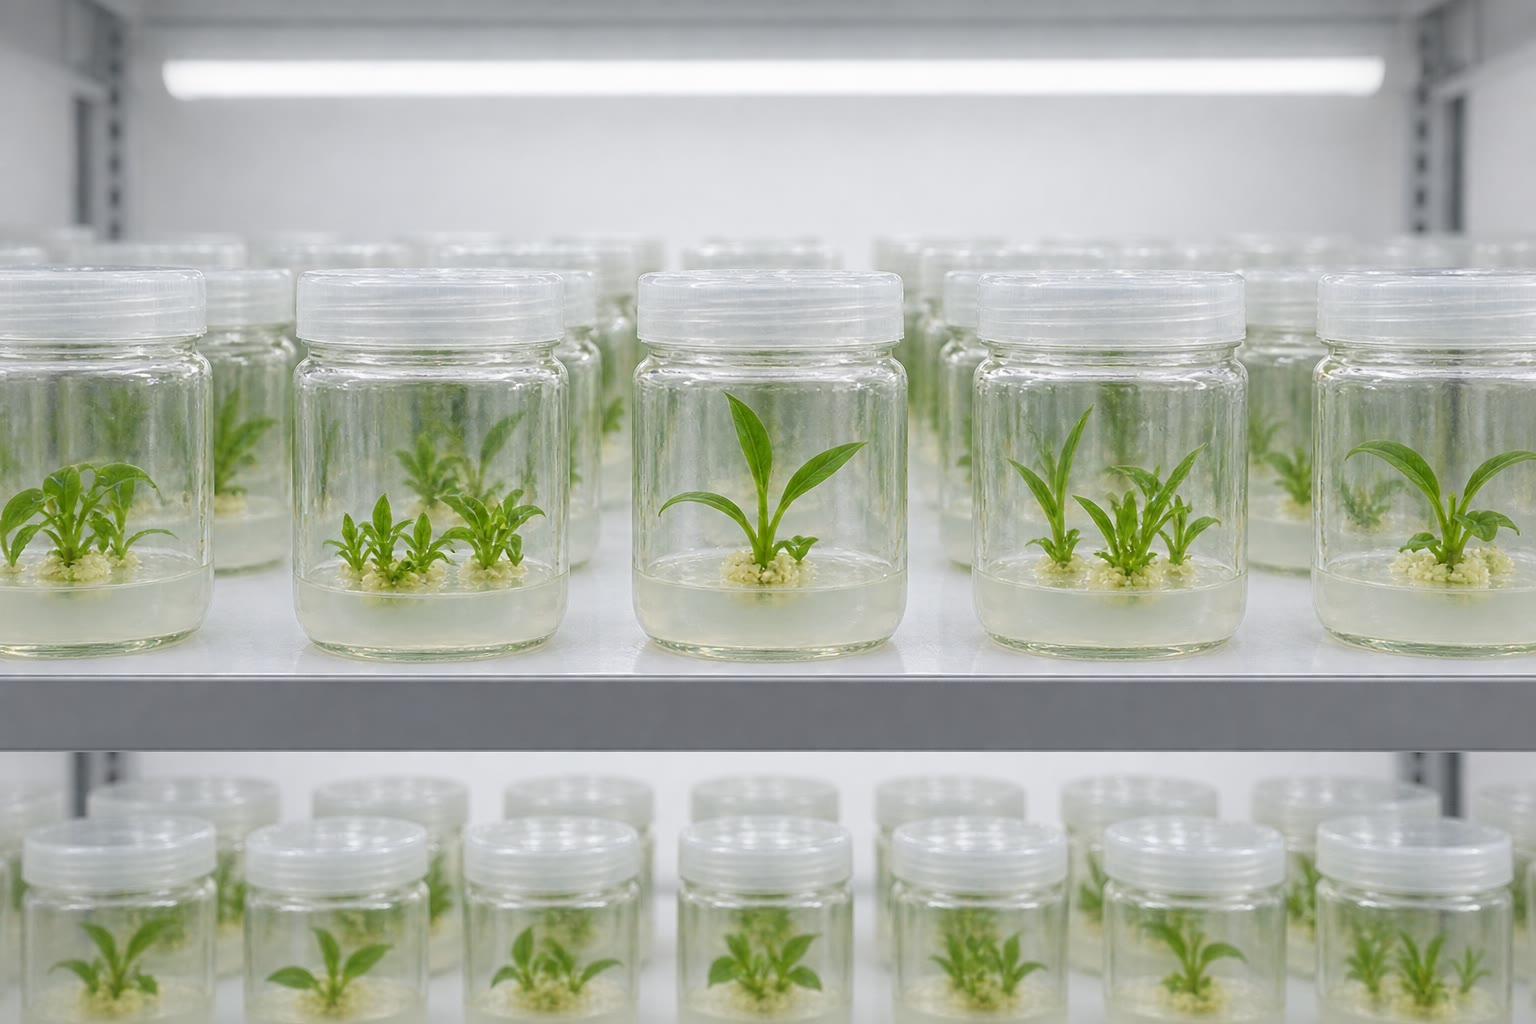
\includegraphics[width=0.6\linewidth]{images/book4/ai/b4-07-tissue-culture.jpg}

{\small Plantjes op agar in een kweekruimte: elke pot bevat een \omterm{def:b2:asexual-reproduction:clone}{kloon} van
hetzelfde ras, vermenigvuldigd uit één meristeem.}
\end{omfigure}

\section{De kosten van seks en de kosten van het zonder doen}

\begin{theorem}[De tweevoudige kosten van seks]\label{thm:b2:asexual-reproduction:twofold}
\index{tweevoudige kosten van seks}
In een populatie waarin vrouwtjes elk $F$ nakomelingen maken, waarvan de
helft zonen zijn, verdubbelt een ongeslachtelijk mutant vrouwtje dat $F$
dochters maakt, allemaal kopieën van zichzelf, haar aandeel in de
vrouwtjes van de volgende generatie. Als de ongeslachtelijke lijn onder de
vrouwtjes frequentie $p$ heeft, dan geldt in de volgende generatie
\[
p' = \frac{2p}{1 + p}, \qquad p_t = \frac{2^t p_0}{1 + (2^t - 1)p_0},
\]
zodat ze van één op duizend in tien generaties de helft van de populatie
bereikt en kort daarna het geheel. Als al het andere gelijk is, halveert
seks het tempo waarmee een lijn zich vermenigvuldigt --- de prijs van het
maken van mannetjes. Aangezien seks toch vrijwel universeel is, is al het
andere niet gelijk: geslachtelijke lijnen moeten gemiddeld minstens een
factor twee winnen uit recombinatie.
\end{theorem}
\begin{proof}
Ongeslachtelijke vrouwtjes zijn met $pN$ en laten $FpN$ dochters na;
geslachtelijke vrouwtjes zijn met $(1 - p)N$ en laten $F(1 - p)N/2$
dochters na (de andere helft zijn zonen, die geen eieren maken). Het
ongeslachtelijke aandeel in de dochters is $Fp/(Fp + F(1 - p)/2) = 2p/(1 + p)$.
Schrijft men $q = p/(1 -
p)$, dan wordt de recursie $q' = 2q$, dus $q_t = 2^t q_0$; terugrekenen
geeft $p_t$. Stelt men $p_t = \tfrac12$, dan is $2^t q_0 = 1$, d.w.z.\
$t = \log_2(1/q_0) \approx 10$ voor $p_0 = 10^{-3}$.
\end{proof}

\begin{omfigure}
\begin{tikzpicture}
\begin{axis}[
  width=0.76\linewidth, height=5.6cm,
  axis x line=bottom, axis y line=left,
  xmin=0, xmax=20, ymin=0, ymax=1.05,
  xlabel={generaties}, ylabel={frequentie van de ongeslachtelijke lijn},
  xlabel style={font=\small, at={(axis description cs:0.5,-0.13)}, anchor=north},
  ylabel style={font=\small},
  tick label style={font=\small}, xtick={0,5,10,15,20}, ytick={0,0.5,1},
  legend style={font=\scriptsize, at={(0.5,-0.3)}, anchor=north, draw=none},
  clip=false,
]
\addplot[very thick, omThm, domain=0:20, samples=80] {2^x*0.001/(1+(2^x-1)*0.001)};
\addlegendentry{geen ander verschil: neemt in 12 generaties over}
\addplot[very thick, omDef, domain=0:20, samples=80] {0.001*(1.3)^x/(1+(1.3^x-1)*0.001)};
\addlegendentry{ongeslachtelijken verliezen \qty{35}{\%} fitness aan parasieten: trager}
\addplot[very thick, omProp, domain=0:20, samples=80] {0.001*(0.9)^x/(1+(0.9^x-1)*0.001)};
\addlegendentry{ongeslachtelijken verliezen \qty{55}{\%}: ze verspreiden zich nooit}
\end{axis}
\end{tikzpicture}

{\small Het tweevoudige voordeel in actie. Vanaf één op duizend neemt een
ongeslachtelijke lijn zonder ander nadeel het in een tiental generaties
over; alleen een fitnessverlies van minstens de helft --- door parasieten,
opgestapelde \omterm{def:b2:genome-diversification:mutation}{mutaties} of tragere aanpassing --- houdt haar tegen.}
\end{omfigure}

\begin{proposition}[Waartoe seks dient]\label{prop:b2:asexual-reproduction:whysex}
\index{ratel van Muller}\index{Rode Koningin-hypothese}
Drie voordelen zijn groot genoeg om ertoe te doen. \emph{De \omterm{prop:b2:asexual-reproduction:whysex}{ratel van
Muller}}: in een \omterm{def:b2:asexual-reproduction:clone}{kloon} wordt elke schadelijke \omterm{def:b2:genome-diversification:mutation}{mutatie} door alle
nakomelingen geërfd, en een mutatievrij genoom dat eenmaal door toeval uit
een eindige populatie is verdwenen, kan nooit opnieuw worden gemaakt; de
last klikt omhoog, één tand tegelijk, en kleine ongeslachtelijke populaties
takelen af. Recombinatie bouwt uit twee beschadigde genomen weer schone
genomen op. \emph{Aanpassing}: twee nuttige \omterm{def:b2:genome-diversification:mutation}{mutaties} die in verschillende
individuen van een \omterm{def:b2:asexual-reproduction:clone}{kloon} ontstaan, wedijveren en één gaat verloren; in een
geslachtelijke populatie worden ze gecombineerd (Fisher en Muller, jaren
1930), zodat geslachtelijke populaties sneller aanpassen wanneer veel genen
moeten veranderen. \emph{De Rode Koningin}: parasieten passen zich aan het
meest voorkomende \omterm{def:b2:meiosis-heredity:vocabulary}{genotype} van de gastheer aan, en een \omterm{def:b2:asexual-reproduction:clone}{kloon}, die één
\omterm{def:b2:meiosis-heredity:vocabulary}{genotype} is, is het meest voorkomende van allemaal; geslachtelijke ouders
maken van elke nakomeling een nieuw slot. Bij slakken, vissen en planten
met zowel geslachtelijke als klonale populaties overheersen de
geslachtelijke populaties waar parasieten talrijk zijn. De ongeslachtelijke
lijnen die floreren --- paardenbloemen, bdelloïde raderdiertjes, de meeste
klonale gewassen --- zijn ofwel jong, ofwel polyploïde hybriden die eigen
variatie meedragen, ofwel overeind gehouden door een teler die hun
parasieten voor hen doodt.
\end{proposition}

\begin{example}[Monoculturen van een kloon]\label{ex:b2:asexual-reproduction:monoculture}
In de jaren 1840 bestond het grootste deel van de aardappeloogst van
Ierland uit één klonaal ras, de Lumper; de oömyceet \emph{Phytophthora
infestans}, die in 1845 aankwam, trof een land vol genetisch identieke,
uniform vatbare planten en vernietigde de oogst drie jaar achter elkaar.
De exportbanaan van de wereld was tot de jaren 1950 één enkele \omterm{def:b2:asexual-reproduction:clone}{kloon}, Gros
Michel, die door een bodemschimmel uit de plantages van Midden-Amerika werd
weggevaagd; zijn opvolger, Cavendish, is eveneens één enkele \omterm{def:b2:asexual-reproduction:clone}{kloon} en gaat
nu, plantage na plantage, verloren aan een nieuwe stam van dezelfde
schimmel, waartegen hij geen variatie te bieden heeft. Een \omterm{def:b2:asexual-reproduction:clone}{kloon} is het
gemakkelijkste doelwit in de natuur, en de teler die er een plant, moet
de resistentie leveren die recombinatie gratis zou hebben geleverd.
\end{example}

\section{Opgaven}

\begin{exercise}[$\star$]\label{exo:b2:asexual-reproduction:1}
Definieer \omterm{def:b2:asexual-reproduction:clone}{kloon}, \omterm{def:b2:asexual-reproduction:clone}{genet} en \omterm{def:b2:asexual-reproduction:clone}{ramet}, en geef drie natuurlijke organen van
\omterm{def:b2:asexual-reproduction:clone}{vegetatieve vermeerdering} met bij elk een plant.
\end{exercise}

\begin{exercise}[$\star$]\label{exo:b2:asexual-reproduction:2}
Welke weefsels moeten bij een ent op elkaar aansluiten opdat de verbinding
slaagt, en wat draagt elke partner bij aan de boom? Waarom is een geënte
boom een chimaera en geen hybride?
\end{exercise}

\begin{exercise}[$\star$]\label{exo:b2:asexual-reproduction:3}
Onderscheid \omterm{def:b2:asexual-reproduction:apomixis}{apomixie} van \omterm{def:b2:asexual-reproduction:clone}{vegetatieve vermeerdering}, en \omterm{def:b2:asexual-reproduction:apomixis}{parthenogenese} van
beide. Welke van de drie behoudt het \omterm{def:b2:angiosperm-reproduction:seed}{zaad}?
\end{exercise}

\begin{exercise}[$\star$]\label{exo:b2:asexual-reproduction:4}
Noem de stappen van microvermeerdering van explantaat tot plant op het
veld, met de hormoonomstandigheden bij elke stap.
\end{exercise}

\begin{exercise}[$\star\star$]\label{exo:b2:asexual-reproduction:5}
Een aardbeienplant maakt 8 uitlopers per jaar, die elk 3 plantjes
bewortelen, en elk plantje doet het jaar daarop hetzelfde. Hoeveel planten
zijn er na 4 jaar als er geen doodgaan? Welke oppervlakte zouden ze nodig
hebben bij \qty{0.1}{m^2} per plant? Wat beperkt de \omterm{def:b2:asexual-reproduction:clone}{kloon} in werkelijkheid?
\end{exercise}

\begin{exercise}[$\star\star$]\label{exo:b2:asexual-reproduction:6}
De populierenkloon Pando heeft \num{47000} stammen op \qty{43}{ha}, en elke
stam leeft ongeveer \num{130} jaar. Als het \omterm{def:b2:asexual-reproduction:clone}{genet} \num{14000} jaar oud is,
hoeveel generaties stammen heeft het dan gehad? Bereken zijn gemiddelde
radiale opmars in meter per jaar, door het als een schijf te behandelen.
\end{exercise}

\begin{exercise}[$\star\star$]\label{exo:b2:asexual-reproduction:7}
Een ongeslachtelijke mutant ontstaat met frequentie $10^{-4}$ in een
geslachtelijke populatie, met dezelfde vruchtbaarheid. Bereken zijn
frequentie na 5, 10 en 15 generaties. Hoeveel moet zijn fitness verlaagd
zijn opdat hij zich nooit verspreidt?
\end{exercise}

\begin{exercise}[$\star\star$]\label{exo:b2:asexual-reproduction:8}
Voorspel wat een tabakscallus doet op media met een verhouding auxine :
cytokinine van 10 : 1, 1 : 1 en 1 : 10, en leg uit waarom een scheutstek in
auxine wordt gedompeld en niet in cytokinine.
\end{exercise}

\begin{exercise}[$\star\star$]\label{exo:b2:asexual-reproduction:9}
Aardappelen worden als knollen gepoot. Een gepote kilogram brengt
\qty{10}{kg} op, en een hectare vraagt \qty{2}{t} pootgoed. Hoeveel
seizoenen duurt het, uitgaande van \qty{1}{kg} van een nieuw ras, voordat
een hectare kan worden beplant? Waarom geeft echt \omterm{def:b2:angiosperm-reproduction:seed}{zaad} een snellere
vermeerdering, maar wordt het niet gebruikt?
\end{exercise}

\begin{exercise}[$\star\star\star$]\label{exo:b2:asexual-reproduction:10}
In een klonale populatie van $N$ individuen met $U$ schadelijke \omterm{def:b2:genome-diversification:mutation}{mutaties}
per genoom per generatie, die elk een fractie $s$ fitness kosten, is de
fractie mutatievrije individuen in evenwicht
$e^{-U/s}$ (afgeleid in \cref{ch:b2:population-genetics}). Bereken met $U =
0.1$ en $s = 0.02$ het aantal mutatievrije
individuen voor $N = 10^{5}$ en $N = 10^{3}$, en leg met de \omterm{prop:b2:asexual-reproduction:whysex}{ratel van
Muller} uit waarom de kleine populatie gedoemd is en de grote niet ---
nog niet.
\end{exercise}

\begin{exercise}[$\star\star\star$]\label{exo:b2:asexual-reproduction:11}
Een pathogeenstam die de resistentie van een bepaald \omterm{def:b2:meiosis-heredity:vocabulary}{genotype} doorbreekt,
ontstaat één keer. Vergelijk zijn lot in een veld met één \omterm{def:b2:asexual-reproduction:clone}{kloon} en in een
geslachtelijke populatie waarin de resistentiegenen op tien loci
uitsplitsen, elk met twee \omterm{def:b2:meiosis-heredity:vocabulary}{allelen} van gelijke frequentie, en verklaar de
Ierse aardappelhongersnood in deze termen.
\end{exercise}

\begin{exercise}[$\star\star\star$]\label{exo:b2:asexual-reproduction:12}
``Seks kost een factor twee en is overal; ongeslachtelijkheid is goedkoop
en zeldzaam.'' Bespreek de drie verklaringen uit het hoofdstuk, en zeg wat
de bdelloïde raderdiertjes --- al veertig miljoen jaar ongeslachtelijk ---
voor elk ervan betekenen.
\end{exercise}

\section{Vraagstuk: een aardbeienkwekerij en een oude kloon}

\begin{problem}[{Weekendvraagstuk --- de rekenkunde van een kloon, van
een aardbeienveld dat zich via uitlopers vult en een laboratorium dat een
meristeem vermenigvuldigt, tot de invasie van een geslachtelijke populatie
door een apomict en het genetische verval van een oeroud genet, met als
besluit de tijd om het veld te vullen, het aantal plantjes uit één
meristeem, en het evenwicht tussen apomicten en geslachtelijke planten}]
\label{pb:b2:asexual-reproduction:1}
Een teler plant \num{100} aardbeienplanten in een veld van
\qty{1}{ha} dat \num{4} planten per vierkante meter kan dragen. Elke
plant maakt \num{6} uitlopers per jaar, die elk \num{2} dochters
bewortelen, en alle planten overleven. Een laboratorium vermenigvuldigt
hetzelfde ras door weefselkweek: elke overzetting, om de \num{4} weken,
vermenigvuldigt de scheuten met \num{5}; \qty{80}{\%} van de plantjes
overleeft het wennen aan de grond. Gewone stekken van het ras zijn voor
\qty{90}{\%} met virus besmet; meristeemtoppen van \qty{0.3}{mm} dragen het
virus met kans
$0.02$. Genoom van de populier: \qty{4.8e8}{} basenparen; somatische
\omterm{thm:b2:genome-diversification:rate}{mutatiesnelheid} \qty{1e-9}{} per basenpaar per celdeling; \num{20}
celdelingen van het meristeem per jaar in een groeiende scheut.

\medskip
\noindent\textbf{Deel I --- Het veld vullen.}
\begin{enumerate}
  \item Hoeveel planten kan het veld bevatten?
  \item Met welke factor vermenigvuldigt het aantal planten elk jaar?
  \item Bereken het aantal planten na 1, 2 en 3 jaar.
  \item Los $N(t) = 100\times 13^{t}$ op naar het tijdstip waarop het veld
        vol is.
  \item Eenmaal vol vinden alleen de planten aan de rand van een plek nog
        ruimte. Als een plek \qty{0.5}{m} per jaar oprukt, hoeveel jaar zou
        één plant er dan over doen om het veld alleen door opmars te
        bedekken?
  \item Leg uit waarom de teler \num{100} over het veld verspreide planten
        plant in plaats van één.
\end{enumerate}

\medskip
\noindent\textbf{Deel II --- Het laboratorium.}
\begin{enumerate}[resume]
  \item Hoeveel overzettingen zijn er nodig om van één meristeem tot
        minstens $10^{6}$ scheuten te komen? Hoeveel weken?
  \item Hoeveel planten overleven het wennen aan de grond?
  \item Wat is de kans dat een lijn uit een meristeem virusvrij is? Dat
        alle \num{10} lijnen die uit één plant zijn gestart het zijn?
  \item Het laboratorium start \num{10} lijnen en verwijdert na een test
        de besmette. Verwacht aantal schone lijnen? Vergelijk met stekken.
  \item Leg uit waarom de meristeemtop aan het virus ontsnapt.
  \item Het veld zou in het eerste jaar met de productie van het
        laboratorium kunnen worden beplant, in plaats van in drie jaar
        via uitlopers te worden gevuld. Geef bij elke route één voordeel
        en één risico.
\end{enumerate}

\medskip
\noindent\textbf{Deel III --- Een apomict dringt binnen.}
Een populatie paardenbloemen is geslachtelijk; een apomictische
(zaadklonende) mutant verschijnt met frequentie $p_0 = 10^{-3}$ en met
dezelfde zaadproductie per plant. De helft van de voortplantingsinspanning
van de geslachtelijke planten gaat naar \omterm{def:b2:plant-life-cycles:heterospory}{stuifmeel}.
\begin{enumerate}[resume]
  \item Verantwoord de recursie $p' = 2p/(1 + p)$ voor de frequentie van
        de apomict onder de zaadouders.
  \item Bereken $p$ na 5 en 10 generaties, en de generatie waarin de
        frequentie de helft passeert.
  \item Een roestschimmel specialiseert zich op het meest voorkomende
        \omterm{def:b2:meiosis-heredity:vocabulary}{genotype}: de zaadproductie van de apomict wordt verlaagd met een
        factor $(1 - cp)$, met
        $c = 0.8$. Schrijf de nieuwe recursie.
  \item Bepaal de evenwichtsfrequentie $p^*$ en controleer haar stabiliteit
        aan de hand van het teken van $p' - p$ aan weerszijden.
  \item Voor welke waarden van $c$ neemt de apomict het volledig over?
  \item Bereken het evenwicht voor $c = 0.6$. Interpreteer: wat moet een
        parasiet doen om seks te beschermen?
  \item De apomict is triploïd. Waarom kan hij niet terug naar seks, en
        waarom doet dit er op lange termijn toe?
\end{enumerate}

\medskip
\noindent\textbf{Deel IV --- De oude \omterm{def:b2:asexual-reproduction:clone}{kloon}.}
\begin{enumerate}[resume]
  \item Bereken het aantal somatische \omterm{def:b2:genome-diversification:mutation}{mutaties} per celdeling bij de
        populier.
  \item Twee stammen van de \omterm{def:b2:asexual-reproduction:clone}{kloon} Pando zijn gescheiden door \num{14000}
        jaar groei aan weerszijden van hun gemeenschappelijke voorouder.
        Hoeveel celdelingen scheiden ze, en hoeveel \omterm{def:b2:genome-diversification:mutation}{mutaties} onderscheiden
        hun genomen?
  \item Welke fractie van het genoom is dat? Als \qty{2}{\%} van het
        genoom coderend is, hoeveel coderende verschillen zijn dat dan?
  \item Een \omterm{def:b2:asexual-reproduction:clone}{kloon} heeft geen \omterm{def:b2:meiosis-heredity:meiosis}{meiose} en geen selectie op het niveau van het
        organisme om deze \omterm{def:b2:genome-diversification:mutation}{mutaties} te verwijderen. Wat verwijdert ze wel,
        en waarom is die zeef zwakker dan in een geslachtelijke lijn?
  \item Is Pando ``genetisch uniform''? Bespreek in twee zinnen.
  \item Formuleer het resultaat: de tijd om het veld via uitlopers te
        vullen, het aantal plantjes dat één meristeem in een jaar geeft, en
        de evenwichtsfrequentie van de apomict voor $c = 0.8$.
\end{enumerate}
\end{problem}
